% flashcards-title: Tangent slope on a velocity-time graph
% flashcards-desc: A curved velocity-time graph has a tangent line at a marked time, separating the graph value from its local slope.
\documentclass[border=7pt]{standalone}
\def\pgfsysdriver{pgfsys-dvisvgm.def}
\usepackage{tikz}
\usetikzlibrary{arrows.meta,positioning,shapes.geometric}
\definecolor{mechInk}{HTML}{172033}
\definecolor{mechBlue}{HTML}{155EEF}
\definecolor{mechOrange}{HTML}{B54708}
\definecolor{mechPale}{HTML}{E8F0FF}
\definecolor{mechGray}{HTML}{667085}
\definecolor{mechLight}{HTML}{D0D5DD}
\tikzset{
  every picture/.style={font=\sffamily\large, text=mechInk},
  mech box/.style={draw=mechInk, line width=1.2pt, rounded corners=4pt,
    fill=white, align=center, minimum height=14mm, inner xsep=5mm},
  mech primary/.style={draw=mechBlue, line width=2.2pt},
  mech secondary/.style={draw=mechOrange, line width=2.2pt, dashed},
  mech guide/.style={draw=mechGray, line width=0.9pt, dashed},
  mech arrow/.style={-{Stealth[length=3.2mm,width=2.4mm]},
    draw=mechInk, line width=1.4pt, line cap=butt},
  mech axis/.style={draw=mechInk, line width=1.2pt},
  mech tick/.style={draw=mechInk, line width=1pt}
}

\begin{document}
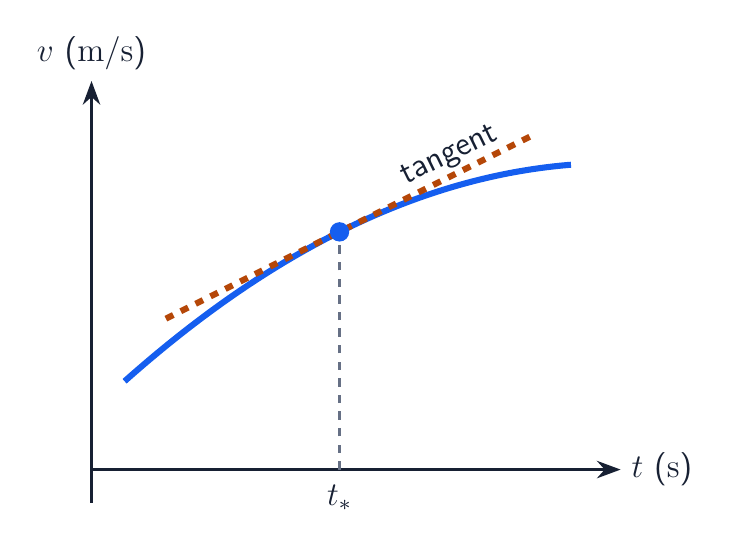
\begin{tikzpicture}[x=1.05cm,y=1.05cm]
  \draw[mech axis,-{Stealth[length=3mm,width=2.2mm]}] (0,0) -- (6.4,0) node[right] {\(t\) (\(\mathrm{s}\))};
  \draw[mech axis,-{Stealth[length=3mm,width=2.2mm]}] (0,-0.4) -- (0,4.7) node[above] {\(v\) (\(\mathrm{m/s}\))};
  \draw[mech primary,domain=0.4:5.8,samples=80,smooth] plot (\x,{0.7+0.95*\x-0.075*\x*\x});
  \coordinate (P) at (3,{0.7+0.95*3-0.075*9});
  \draw[mech secondary] (0.9,{2.875-0.5*2.1}) -- (5.3,{2.875+0.5*2.3});
  \draw[mech guide] (3,0) -- (P);
  \fill[mechBlue] (P) circle (3.5pt);
  \node[below=2pt] at (3,0) {\(t_*\)};
  \node[rotate=26,above] at (4.45,3.55) {tangent};
\end{tikzpicture}
\end{document}
